% -*- coding: utf-8 -*-

\section{Rectangular Swept Spheres}
\label{rss}

\subsection{Introduction}
In this section I will go into greater detail about the RSS, how it is defined and represented, as well as the literature that I have used in this report. I will also shortly describe Point Swept Spheres (PSS) and Linear Swept Spheres (LSS), which are related to RSS'. No other bounding volumes will be described. 

\begin{figure}
\centering
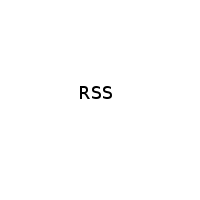
\includegraphics[\width=0.5\textwidth]{figures/rss}
\caption{\label{rss-example}An example of a RSS}
\end{figure}

\subsection{Rectangular Swept Sphere}
The Rectangular Swept Sphere (RSS) is a 3D figure. It is generated by taking a sphere with a non-zero radius and sweeping it over a rectangle in 3 dimensional space. This makes it reaking it resemble a rectangular rounded pillow. An illustration of a RSS can be found in figure \ref{rss-example}. 

\subsection{Representation of RSS}
I have chosen to represent the RSS as a rectangle in 3D together with a radius, as described in \cite{larsen00fast}, \cite{Larsen99fastproximity} and \cite{237244}. See section \ref{rectangle3d} page \pageref{rectangle3d} for  implementation details. I felt this was best way to represent it, as it adequately described the RSS, took up a minimum of space, contains the vectors, and follows the representation found in \cite{237244}, which is useful, as I use the axis-separation test described in the article.

\subsection{Overlap of 2 RSS'}
\Sfixme{think about whether this is important enough to warrent a section and if so mention how we find out when 2 RSS' are intersecting}


\begin{figure}
\centering
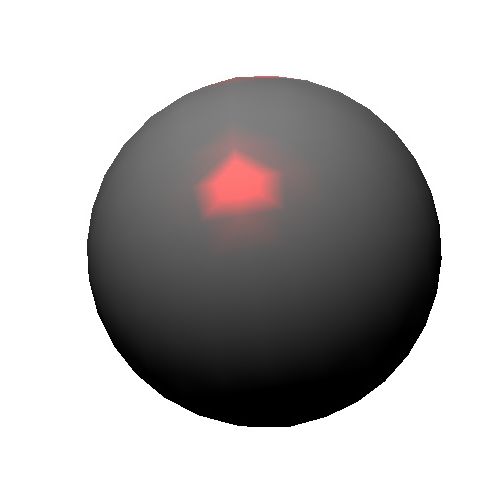
\includegraphics[\width=0.5\textwidth]{figures/pss}
\caption{\label{pss-example}An example of a PSS}
\end{figure}

\subsection{Point Swept Spheres}
A point swept sphere is a BV that is created by taking a point p in 3D, and placing the center point of a sphere s with a positive radius at p. The advantage of the PSS is that it is both simple to implement and to check to for intersection with other PSS. PSS do however not have a very tight fit, and is therefore likely to necesitate more intersection checks in practice, than other BVs, such as LSS' (se below) or RSS'.\Sfixme{Do I have to argument for this claim, and if so, which arguments can I use}

\begin{figure}
\centering
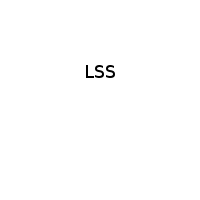
\includegraphics[\width=0.5\textwidth]{figures/lss}
\caption{\label{lss-example}An example of a LSS}
\end{figure}

\subsection{Linear Swept Spheres}
A linear swept sphere is a BV that is created by taking a line l, placing the center point of a sphere s with a positive radius on one of the endpoints of l, and then sliding s to the other endpoint of l. It is a bit harder to check for intersection for LSS' than it is for PSS' (se above), but LSS will often in practice have a tighter fit to the points it contains, and will therefore create fewer unneeded checks for intersection than PSS'.\Sfixme{Do I have to argument for this claim, and if so, which arguments can I use}
